\chapter{Data Acquisition}\label{ch:data-acquisition}

% multilingual
% - AO3       Cuntz-Leng2015AGermany, Duggan2020WhoAO3, Kleindienst2020InvestigatingSupernatural, Schmidt2022AnalyzingOwn
% - FF.net    Milli2016BeyondFanfiction, Vilares2019HarryLanguage
% - Wattpad   Fast2016ShirtlessCommunity, Liu2019DENS:Analysis, Zhang2019GeneratingFiction

% german
% - FF.de     Cuntz-Leng2015AGermany

In previous research multilingual archives such as \emph{Archive of Our Own}~\citep{Duggan2020WhoAO3, Cuntz-Leng2015AGermany, Kleindienst2020InvestigatingSupernatural, Schmidt2022AnalyzingOwn}, \emph{Fanfiction.net}~\citep{Milli2016BeyondFanfiction, Vilares2019HarryLanguage}, \emph{Wattpad}~\citep{Fast2016ShirtlessCommunity, Liu2019DENS:Analysis, Zhang2019GeneratingFiction} were the objects of study, while only \citet{Cuntz-Leng2015AGermany} gathered some statistical data from \emph{FanFiktion.de}, a german fan fiction website.
As can be seen, little to no research has been done in the field of German fanfiction, despite \citeauthor{Cuntz-Leng2015AGermany}$'$s~\citeyearpar{Cuntz-Leng2015AGermany} emphasis on the importance and opportunities afforded by the study of culturally diverse texts.
For this reason, we dedicated ourselves to the task of assembling and then analyzing a comprehensive corpus consisting exclusively of German fan fiction.


\section{Sources Evaluation}\label{sec:sources-evaluation}
First, we had to locate and evaluate all potential sources of fan fiction texts.
We looked at the languages provided, the number of stories (at the time of collection), the metadata provided, and whether scraping was allowed and feasible under the terms of service of each source.
Table~\ref{tab:evaluation-results} shows an excerpt of the evaluation results (see attachment for a comprehensive table).
% TODO: reference to sources table in attachments

\begin{table}[htp]
%    \renewcommand{\arraystretch}{1.5}
    \centering
%    \begin{tabular}{lllll}%{*{5}{p{15mm}}} % 5x p{15mm}
%    \begin{tabular}{*{5}{p{15mm}}} % 5x p{15mm}
%    \begin{tabular}{|l|l|l|l|l|l|} % adds a vertical spacing
    \begin{tabular}{p{3.4cm}p{2.5cm}p{2cm}p{2cm}p{2cm}} % PAGEWIDTH = 11.9
        \toprule
        \textbf{Name}                                                                                               & \textbf{Language/s} & \textbf{German Stories} & \textbf{Scraping Permitted} & \textbf{Usable} \\
        \midrule
        FanFiktion.de\footnote{https://www.fanfiktion.de/ with TOS https://www.fanfiktion.de/p/terms-of-service/0/} & German & 412.033 & Yes & Yes \\
        FanFiction.Net\footnote{https://www.fanfiction.net/ with TOS https://www.fanfiction.net/tos/} & Multilingual & N/A$^\star$ & No & No \\
        AO3\footnote{https://archiveofourown.org/ with TOS https://archiveofourown.org/tos/} & Multilingual & N/A$^\star$ & Yes & Yes \\
        wattpad\footnote{https://www.wattpad.com/ with TOS https://policies.wattpad.com/terms/} & Multilingual & 1.600 & No & No \\
        tumblr\footnote{https://www.tumblr.com/ with TOS https://www.tumblr.com/policy/en/terms-of-service/} & Multilingual & N/A$^\star$ & No & No \\
        \bottomrule
    \end{tabular}
    \caption[Results of the fan fiction source evaluation.]{Results of the fan fiction source evaluation. (${}^\star$not available; Acquisition date: January 8, 2022)}
    \label{tab:evaluation-results}
\end{table}

Sources were examined according to their provided languages, number of German stories, structure, genres, story metadata, review existence, user information and finally whether scraping is allowed due to the terms of service (TOS).
As seen in Table~\ref{tab:evaluation-results} \emph{FanFiction.NET}, \emph{wattpad} and \emph{tumblr} were excluded from the list of possible candidates for our corpus.
Although \emph{FanFiction.NET} would have been an ideal candidate for inclusion in our corpus with its substantial amount of German text (estimated only), story and user information, and structure in general, scraping in any form is prohibited.
\emph{wattpad} and \emph{Tumblr} were poorly structured, could not be filtered by language or had too few stories in German, had little to no metadata on individual stories, and again, where not allowed to scrape.
Both \emph{Archive of Our Own} and \emph{FanFiktion.de} offered a solid site structure, a large amount of German texts and rich metadata.
While \emph{FanFiktion.de} allowed scraping for non-commercial purposes, \emph{Archive of Our Own} allowed it as long as it did not interfere or disrupt with their services.

Accordingly, \emph{Archive of Our Own} and \emph{FanFiktion.de} are getting used as source material for our corpus and will be referred to as \emph{AO3} and \emph{FF.de}, respectively, in the following paragraphs.

% AO3 descibes itself as a non-commercial archive for transformative fan fiction
% AO3 texts marked as german by the author/s
% AO3: how many german texts compared to total?

Now that the sources could be determined, the next step was to decide which tool to use to obtain the data from the websites.


\section{Web Scraper}\label{sec:web-scraper}

First, the difference between the terms \emph{web crawling} and \emph{web scraping} should be clarified.
While \emph{web crawling} is about finding and discovering URLs or links from websites, \emph{web scraping} is about extracting specified data from websites~\citep{Kenny2022WebCrawling}.
Usually both procedures are needed: first to crawl the URLs of a website and second to scrape the content.

There is a wide range of tools for crawling and scraping the internet.
Factors such as customizability, scalability, the type of input data to be processed, the desired output format, the crawling interval, and the amount of data transferred in the process all play a role.
% what is the input (html)
% what is the output (database)
% what in the scraping interval (continuously)
% how much data (much)
Since we planned to scrape continuously and free of charge, Software as a Service (SaaS) platforms like \emph{ScrapingBee}\footnote{https://www.scrapingbee.com/} or \emph{Diffbot}\footnote{https://www.diffbot.com/} were not suitable.
Desktop scraper applications such as \emph{ScrapeBox}\footnote{https://www.scrapebox.com} were due to the lack of customizability impractical.
In contrast to SaaS and desktop scraper applications, frameworks like \emph{Scrapy}\footnote{https://scrapy.org/}, \emph{Beautiful Soup}\footnote{https://www.crummy.com/software/BeautifulSoup/}, \emph{pyspider}\footnote{http://docs.pyspider.org/en/latest/}, \emph{Goutte}\footnote{https://github.com/FriendsOfPhp/Goutte}, \emph{Cheerio.js}\footnote{https://cheerio.js.org/} and \emph{Puppeteer}\footnote{https://pptr.dev/} were all open source, highly adaptable and scalable, and therefore applicable to our purposes.

\subsection{Scrapy}\label{subsec:scrapy}

We have chosen \emph{Scrapy} as scraping framework because of aspects like those requirements mentioned in the previous section.
\emph{Scrapy} uses the \emph{Python}\footnote{https://www.python.org/} language, is open source, platform-independent, actively maintained, well documented, highly scalable, and got in general lots of features that solve the most common web scraping problems.
Furthermore, one can easily add extensions like proxies and fake user-agents for the obfuscation of queries, or auto-throttle capabilities for adjusting request delays based on the sites current download latency.
Auto-throttle is a particularly valuable feature for not disrupting the sites services while also being able to automatically increase the work load at low usage times, as this was for example requested by \emph{AO3} (see Section~\ref{sec:sources-evaluation}).

\begin{figure}[htp]
    \centering
    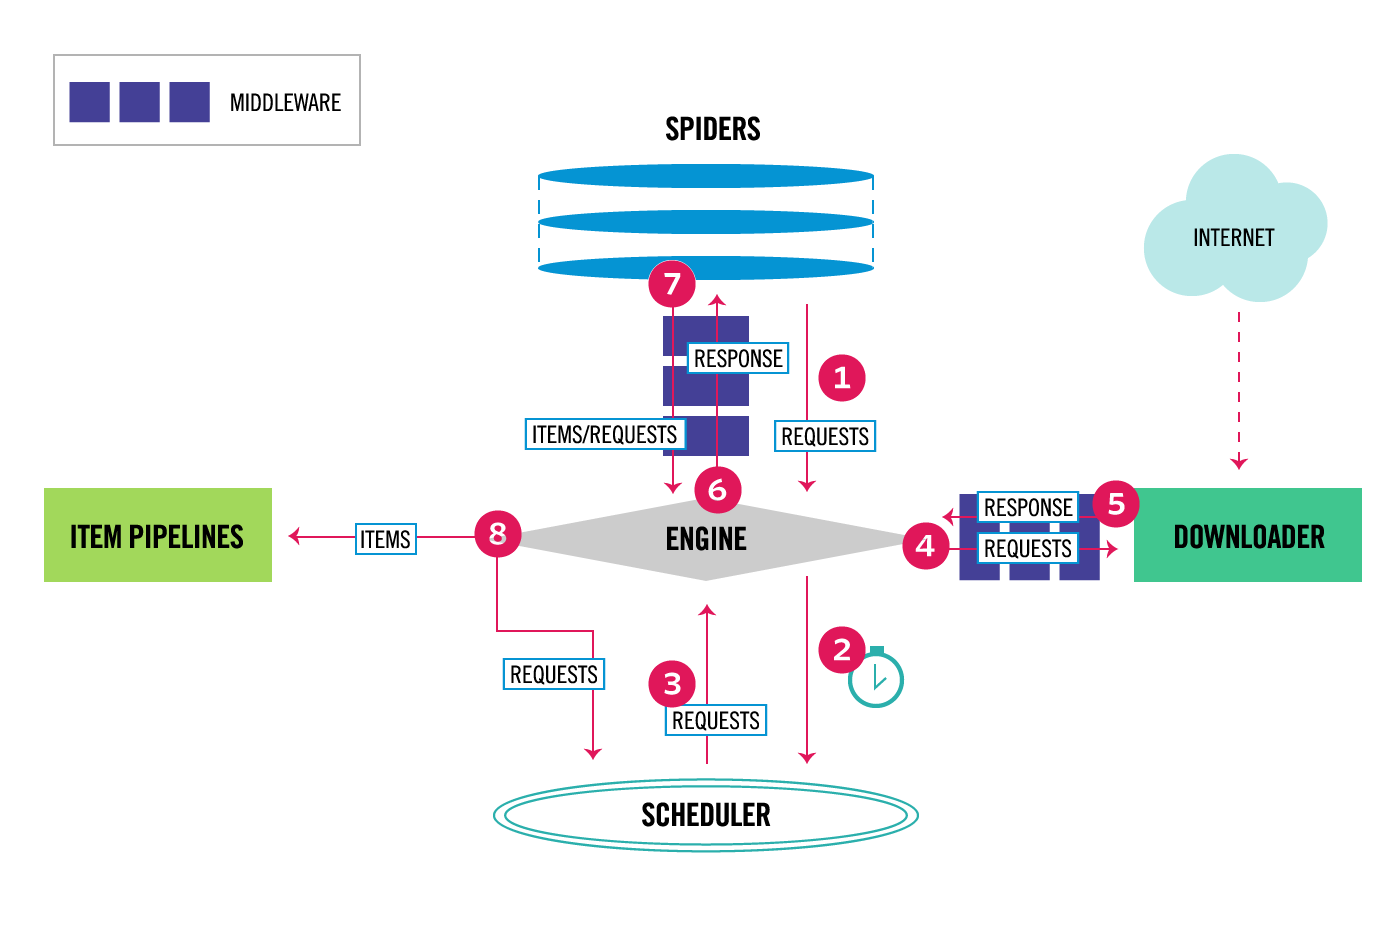
\includegraphics[width=\textwidth]{figures/scrapy_architecture}
    \caption[The architecture of the \emph{Scrapy} framework.]{The architecture of the \emph{Scrapy} framework.
    Reprinted from Architecture overview,
    In Scrapy, n.d., Retrieved October 29, 2022, from https://docs.scrapy.org/en/latest/topics/architecture.html.
    Copyright 2008–2022 by Scrapy developers.}
    \label{fig:scrapy-architecture}
\end{figure}

Figure~\ref{fig:scrapy-architecture} describes the architecture and work flow of the \emph{Scrapy} framework.
Each fan fiction archive, \emph{FF.de} and \emph{AO3}, differs in its page structure and data presentation.
It requires an individual definition of where to find the corresponding data and how to search the respective archive.
These definitions are implemented in so-called \emph{Spiders}.
The \emph{Spider} sends a request with retrieval information via the \emph{Engine} to the \emph{Scheduler}, which stores these requests and forwards them to the \emph{Downloader} with a defined delay (fixed or by using auto-throttle).
The \emph{Downloader} returns the found \emph{Items} to the \emph{Item Pipeline} if successful, where some previously programmed cleanup operations are performed and the objects are stored in a database.

The crawl process runs in a way that the \emph{Spider} seeks and follows a URL for the next page at defined positions.
To filter on a language, headers with appropriate filters must be passed to the request.

% maybe a bit more detailed

\subsection{Concurrent Crawling}\label{subsec:concurrent-crawling}

For time efficiency, we developed and ran two \emph{Spiders}, each with its own public IP, to operate on different hosts at the same time.
Each host was assigned a different fan fiction genre to crawl so that a web page did not have to be processed multiple times.
Since the database for storing the scraped data was only local, we needed a different approach for the remote host.

While the local host's \emph{Spider} stored the data directly in the database, the remote host downloaded the full HTML page, compressed it into an archive (in stacks of 1000 files), and kept a CSV list of the archive's contents.
As per previous definition in Section~\ref{sec:web-scraper}, the local host crawled and subsequently scraped the data, while the remote host merely crawled the URLs and downloaded the web page.

The CSV manifest in each archive contained a list of the names of the downloaded HTML files, the source URLs, the internal IDs of the items (stories, chapters, users or reviews;
see~\ref{subsec:db-schema}), and the chapter number (if applicable).
This list could then be used to skip URLs that had already been processed by searching for the URL found by the crawler.
The HTML files in combination with the CSV files could then be scraped by another spider without any time delay, since the data did not have to be downloaded from a website.


\section{Data Storage}\label{sec:data-storage}

Just like with the web scraper tools, we had to decide on a suitable data storage format.
We needed a storage format that would allow us to store large amounts of data in a well-structured, performant and analyzable way.
Data sets had to be easily supplemented, while avoiding duplicates and data loss.

\subsection{MongoDB}\label{subsec:mongodb}
We used \emph{MongoDB}\footnote{https://www.mongodb.com/} as database for storing the scraped data.

\emph{MongoDB} is a \emph{NoSQL}, non-relational database and has several advantages over few disadvantages for this project.
Data is stored in documents in a \emph{BSON} format which is a \emph{JSON}-like format (see Figure~\ref{fig:bson-document}).  % https://www.mongodb.com/advantages-of-mongodb

\begin{figure}[htp]
    \centering
    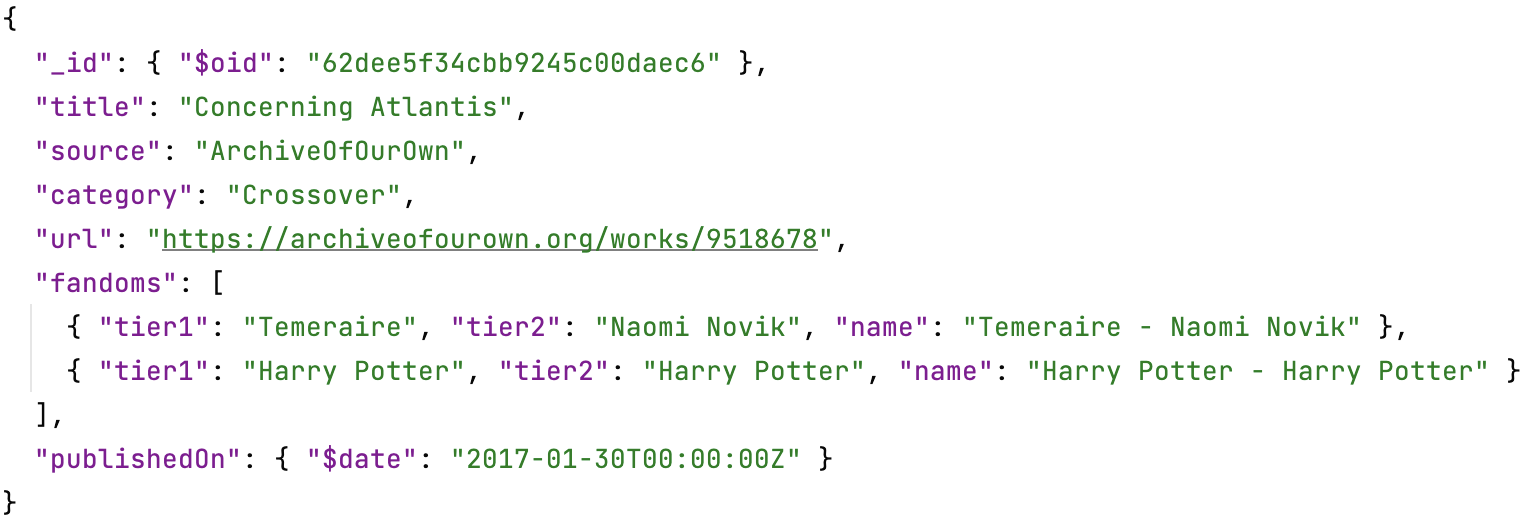
\includegraphics[width=\textwidth]{figures/bson_document}
    \caption[Excerpt of an exemplary story document in the \emph{BSON} format.]{Excerpt of an exemplary story document in the \emph{BSON} format.}
    \label{fig:bson-document}
\end{figure}

These documents are extremely flexible and can store any data without the risk of losing data because the wrong format was used~\citep{Bruce2021UnderstandingMongoDB}.
Unlike with relational database management systems (\emph{RDBMS}), which usually store the data in the 3rd normal form, \emph{NoSQL} databases generally do not use normalized forms~\citep{Chapple2022TheNormalization}.
\emph{MongoDB's} design philosophy states that data should be embedded rather than referenced, resulting in extremely efficient and performant queries since there are no expensive join queries~\citep{MongoDBAdvantagesMongoDB}.

These embeddings lead to redundancies and thus to a higher storage requirement, which is, however, negligible due to the constantly decreasing storage prices~\citep{McCallum2022HistoricalStorage}.
The schemaless structure can also cause data clutter and loss of data quality.

In addition, \emph{MongoDB} with their \emph{BSON}-documents features an easily accessible format for any programming language without the need for object-relational mappers (\emph{ORMs})~\citep{Bruce2021UnderstandingMongoDB}.
The aggregation pipeline can be utilized to build high-performance queries where data is queried and processed in multiple stages~\citep{MongoDBAggregationPipeline}.
Each stage processes its input documents and forwards them to the next stage.
For example, documents can be first filtered, then grouped, and finally sorted, with changes to the output data possible at each of these stages.

\subsection{MongoDB Schema Design}\label{subsec:db-schema}

For data acquisition, we first designed a different database schema than what was later used for the data analysis.

\minisec{Data Acquisition Schema}
Although not in compliance with the design philosophy of mongodb~\citep{MongoDBAdvantagesMongoDB}, this schema rather aligned to the principles of the 3rd normal form common in relational database models.
An excerpt of this can bee seen in Figure~\ref{fig:fan-fiction-db-acquisition-overview} while detailed database model schema can be viewed in Chapter~\ref{ch:appendices}.

% TODO: add comprensive acquisition schema to appendix

\begin{figure}[htp]
    \centering
    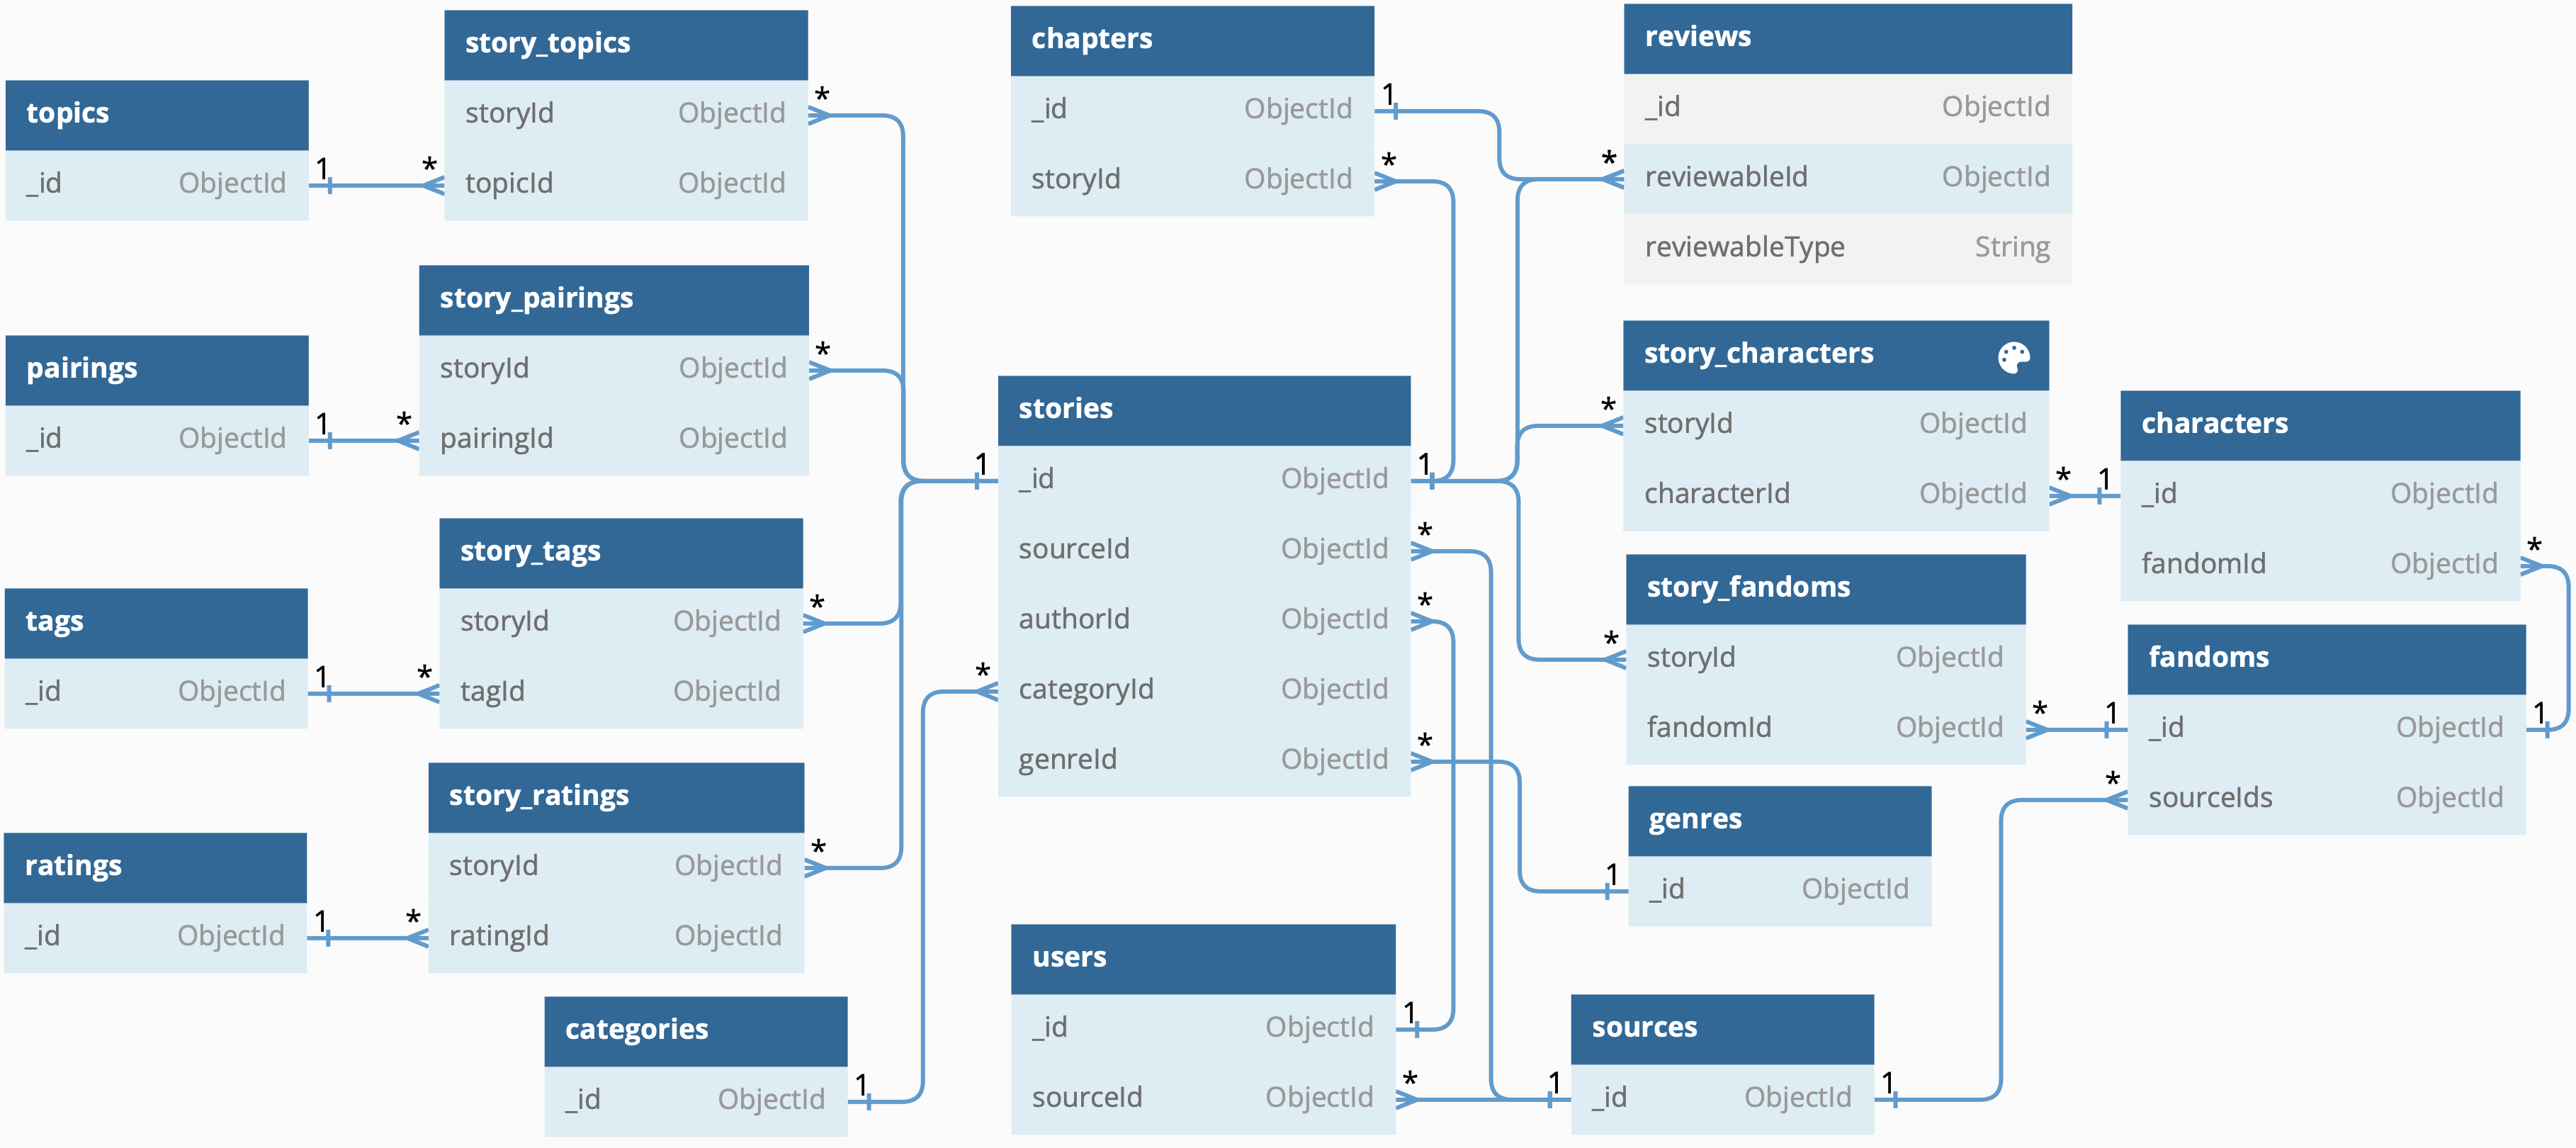
\includegraphics[width=\textwidth]{figures/fan_fiction_db_acquisition_overview}
    \caption[Excerpt of the database schema for the data acquisition.]{Excerpt of the database schema for the data acquisition.}
    \label{fig:fan-fiction-db-acquisition-overview}
\end{figure}

This relational structure had the advantage that, on the one hand, duplicates could be avoided and, on the other hand, data could be cleansed and merged more easily later.
For example, this allowed defining alternative names that are specific to each source archive.
These could be translations (e.g.~the genre could be \emph{Bücher} for \emph{FF.de} and \emph{Books \& Literature} for \emph{AO3}) or differentiating designations (e.g.~the stories pairing could be \emph{MaleSlash} for \emph{FF.de} and \emph{M/M} for \emph{AO3}).
In this way, it was possible to check during the acquisition process whether an item already existed.
Furthermore, if a fandom was to be renamed, this only had to be done in one place.
Both data quality and a consistent presentation and structure could thus be ensured.

\minisec{Data Analysis Schema}
To benefit from the capabilities of MongoDB to the full extent, we subsequently restructured the schema for analyzing the data.

Fields that were specifically needed for the scraping process were removed.
These were, for example, fields that compared the total number of chapters in the story, as indicated in the story overview, with the number of chapters already scraped, without having to query the database each time.
When a story was created in the database, an author was required.
Therefore, we initialized an empty author that contained only a user url and ID for referencing, and set a field for that user indicating that it was provisional and needed to be scraped later in the process.

All the information were then merged into four tables: \emph{stories}, \emph{chapters}, \emph{users} and \emph{reviews}.
An overview of this database schema is illustrated in Figure~\ref{fig:fan-fiction-db-analysis-comprehensive}.
%While an overview of this is illustrated in Figure~\ref{fig:fan-fiction-db-analysis-overview}, a comprehensive illustration can be found in Chapter\ref{ch:appendices}.
The chapter table contained the largest documents, since they stored the entire narrative of a story and were due to \emph{BSON}$'$s size limitation of 16 megabytes not merged into their story document.

% TODO: add comprensive analysis schema to appendix

\begin{figure}[htp]
    \centering
    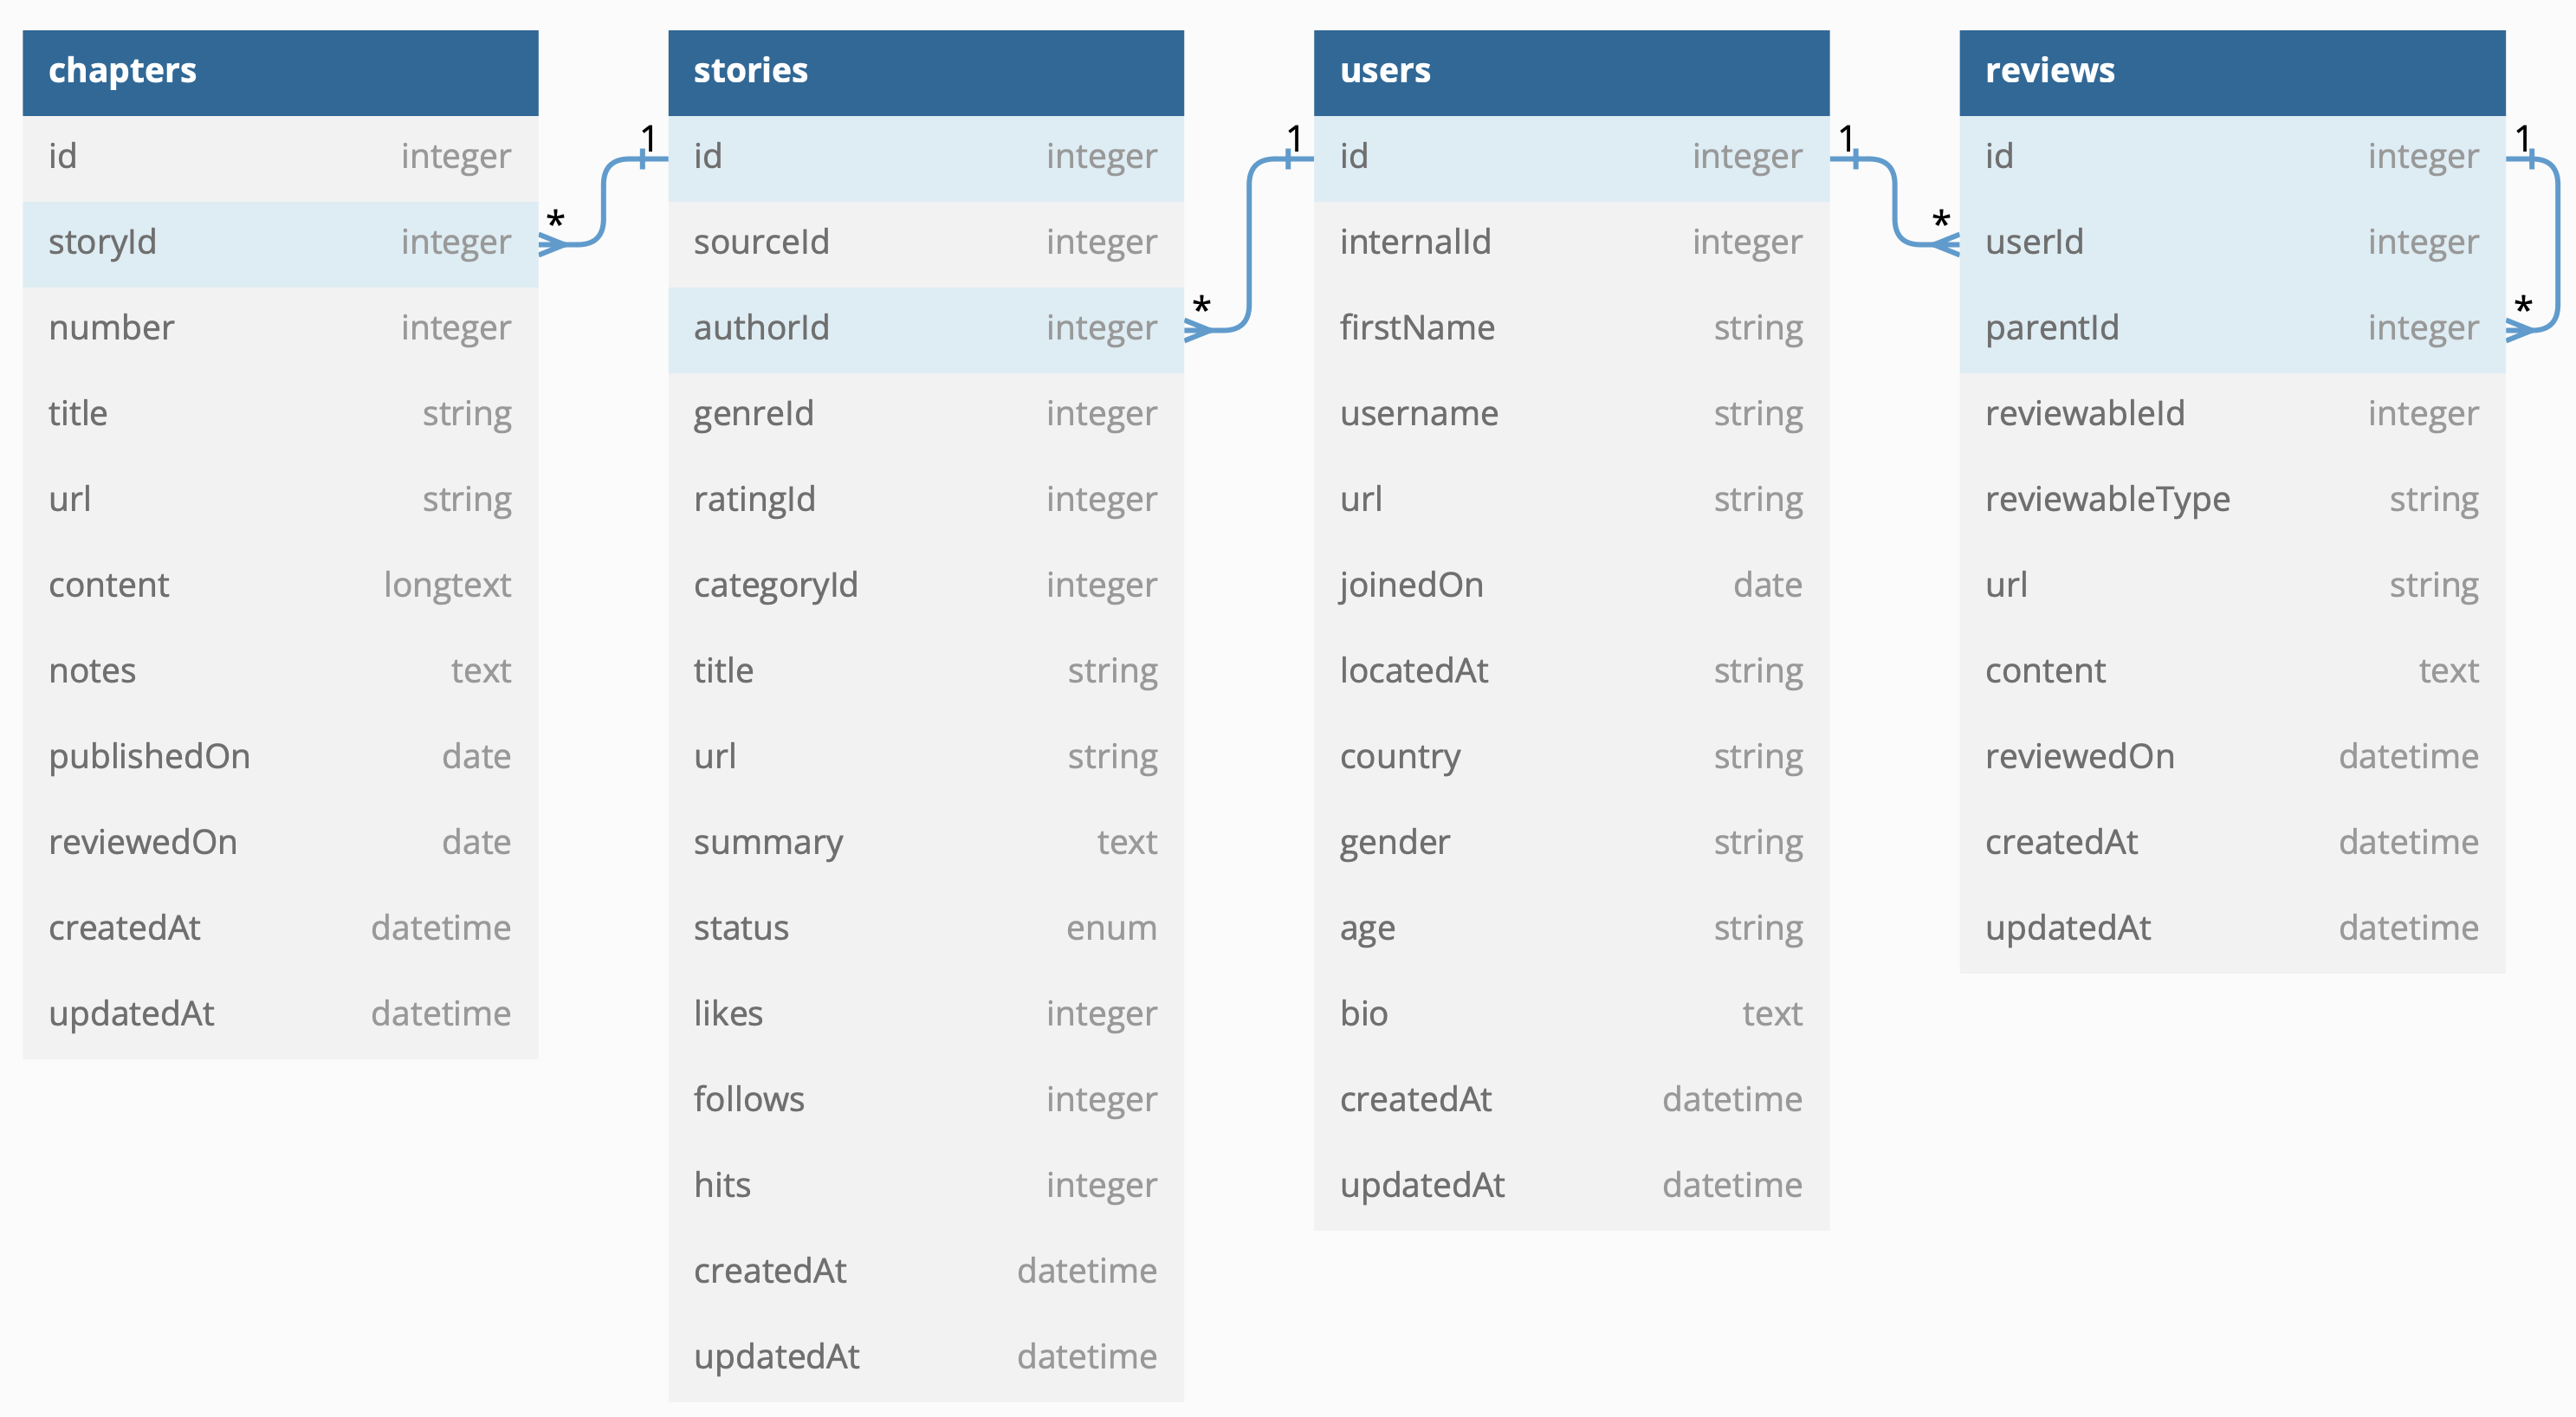
\includegraphics[width=\textwidth]{figures/fan_fiction_db_analysis_comprehensive}
    \caption[Database schema for the data analysis.]{Database schema for the data analysis.}
    \label{fig:fan-fiction-db-analysis-comprehensive}
\end{figure}

As can be seen, this schema is much leaner than the previous one.
Fields from other tables were joined into data structures such as arrays and dictionaries, disregarding the concept of avoiding duplicates.

Characters from a story were consolidated into an array containing the character name as well as the fandom the character originates from.
We structured the fandoms referenced in a story into tiers to allow easier analysis of popular fandoms with many subgenres as illustrated in Figure~\ref{fig:refactor-fandom-example}.

\begin{wrapfigure}{R}{0.65\textwidth}
    \centering
%    \textcolor{lightgray}{\frame{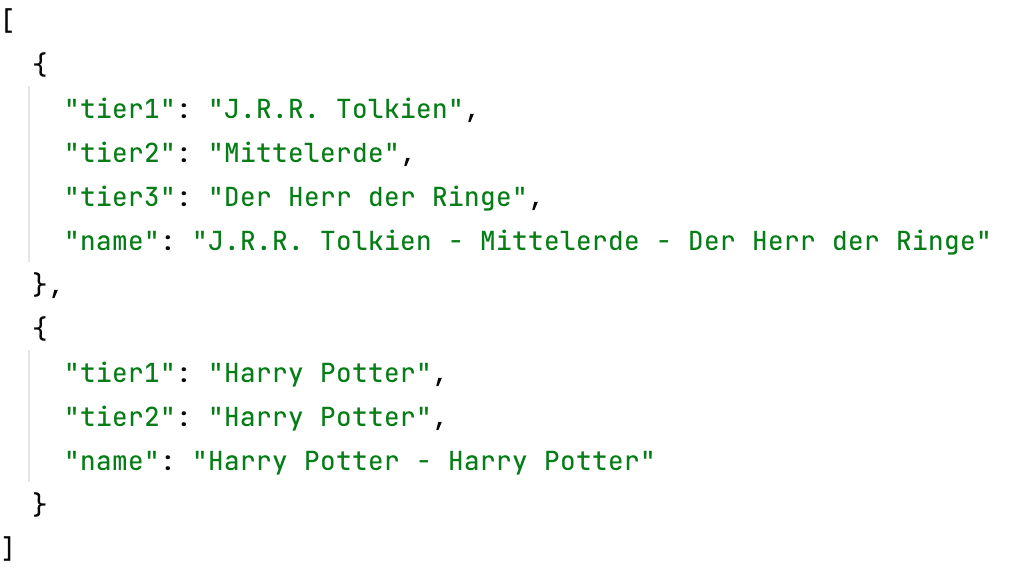
\includegraphics[width=0.4\textwidth]{figures/refactor_fandom_example}}}
    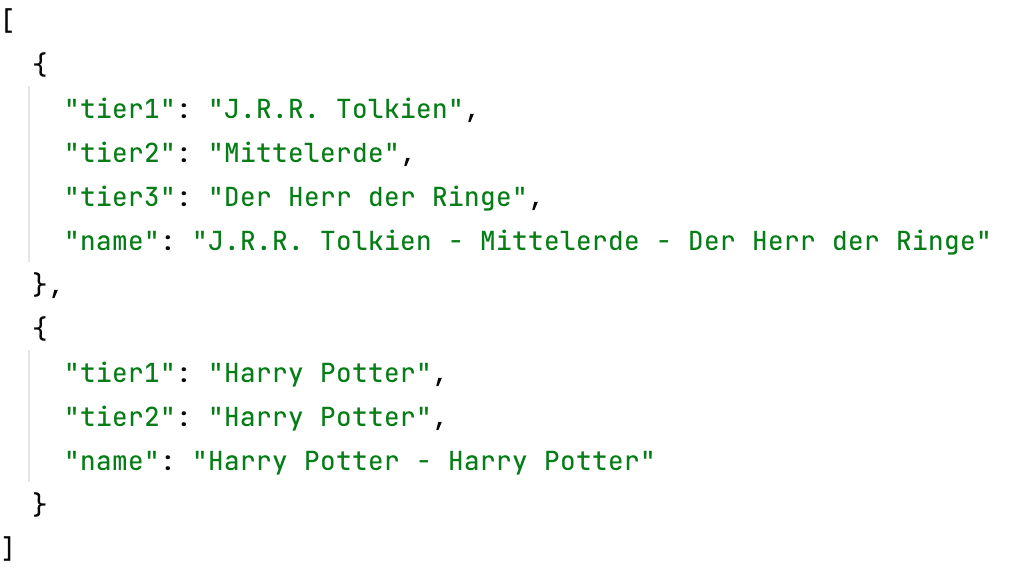
\includegraphics[width=0.6\textwidth]{figures/refactor_fandom_example}
    \caption[Example of refactored story fandoms.]{Example of refactored story fandoms.}
    \label{fig:refactor-fandom-example}
\end{wrapfigure}

\subsection{Cleansing and Plugging Data Holes}\label{subsec:cleansing-data}
In the next step of the data acquisition phase we had to fill in missing data.
This was done by implementing another set of \emph{Spiders}, one for the \emph{AO3} archive and one for the \emph{FF.de} archive.
These \emph{Spiders} were used for data that was missing from the initial scraping process by querying the database for stories and chapters that contained no content or missed other crucial elements like fandom or genre and then scraping it from the archive's website.
After scraping the missing information we still had some stories that contained no text which is why we implemented another, very simple scraper using the \emph{BeautifulSoup} library.
For that we used the URLs referencing the stories from the database and stored the obtained texts.

Numerous stories are published that contain merely an image (e.g.~a cartoon), an embedded video or audio player, a link to a story on another platform or a link to a \emph{YouTube}\footnote{https://www.youtube.com/} video.
Story chapters containing those or did not reach a specified character threshold of 15 characters were removed from the database.
Additionally, low character chapters were manually checked for their content since sometimes rather short but totally valid phrases like ``nicht schwanger'' (german for ``not pregnant'') were used while others were just placeholders.
Stories that subsequently did not include any chapters were also removed from the database.

To improve the quality of the data and increase analyzability, we have consolidated fandoms from both archives under a common name.
For the comparison of fandom names, any punctuation, whitespaces, tabs, line breaks or carriage returns were temporarily removed.
We then used the Levenshtein distance~\citep{Levenshtein1966BinaryReversals}, a metric that measures the difference between two strings based on the minimum number of single character edits such as insertions, deletions or substitutions, to determine the best match from the other archive.
For overview and manual correction, all fandoms of \emph{AO3} were then listed in a table and the most likely counterpart for each based on previous calculations was suggested.
Finally, these values were used for the consolidation in the database.

\section{Difficulties during Data Acquisition}\label{sec:difficulties-acquisition}
We had several problems when collecting the data.

The first problem was that the number of requests per minute to the archives was limited, and we needed to probe the sites for the least time delay between requests possible without being blocked by the host.
Because of the time delay and the huge amount of data available, the scraping process took its time.
To improve this, we ran a second web crawler on another machine, as described earlier in Subsection~\ref{subsec:concurrent-crawling}.
While this reduced the overall time required for scraping, it created another problem in that the fanfiction data was stored in a local database and access from this second computer was therefore not possible, so we used the CSV file as a temporary storage.

Another issue was the age restrictions for certain stories.
While this was handled at \emph{AO3} by confirming the age of majority in a popup window, at \emph{FF.de} we had to either restrict scraping of restricted stories to between 11pm and 4am, or prove our user's age with a valid ID\@.
This could be handled after authentication via \emph{Scrapy}$'$s cookie middleware, where we attached our user's session to the requests.
Sessions, on the other hand, expired after a certain time, and the stories had to be marked as age-restricted for later scraping.

\emph{AO3} distinguishes between fandoms from different media (e.g.~\emph{Sherlock Holmes \textbf{TV}} and \emph{Sherlock Holmes \textbf{Books}}), while \emph{FF.de} is much stricter in this regard and only allows one type of media (e.g.~just \emph{Sherlock Holmes}).
Consolidating the fandoms as outlined in the previous Subsection~\ref{subsec:cleansing-data} solved this issue.

Another difficulty arose from the unreliability of the users.
For example, sometimes authors used the title input box to enter the text of the story, which resulted in documents having empty chapters and overfilled titles.
These stories then had to be scraped anew after they were identified.

% AO3: non-commercial archive for transformative fanfiction
% filtered texts with links, images and (almost) empty
% Due to legal issues the corpus is currently only available upon request via e-mail (thomas.schmidt@ur.de). Reference github?